\begin{surferPage}[المخروط المزدوج]%
{المخروط المزدوج}
كما شرحنا في مقدمة هذه الجاليريا، نتكلم عن منحني \emph{أملس }حين لا يكون له نتوءات (والتي تٌسمى متفردات).
   هذه هي الحال مع كرة أو مع حلقة (الصورتان أدناه في الطرف ):
    \begin{center}
      \begin{tabular}{@{}c@{}c@{}c@{}c@{}}
        \begin{tabular}{@{}c}
          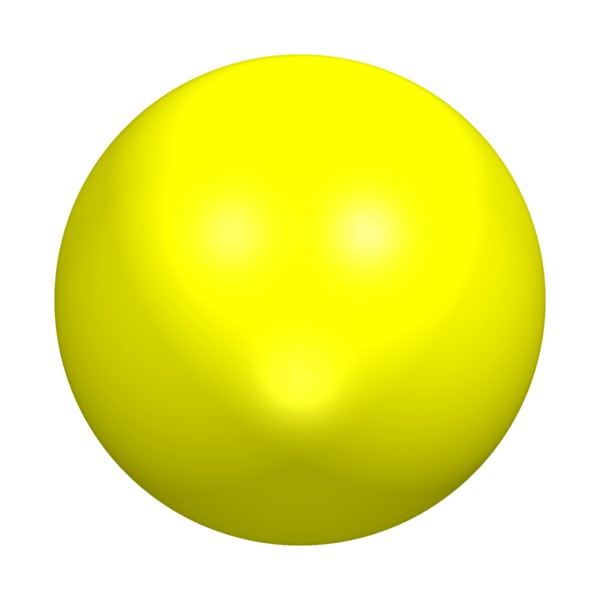
\includegraphics[width=1.4cm]{kugel}
        \end{tabular}
        &
        \begin{tabular}{@{}c}
          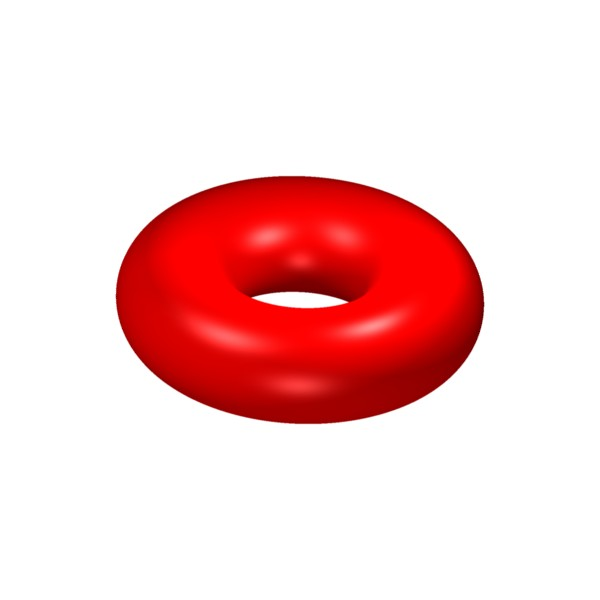
\includegraphics[width=1.4cm]{torus}
        \end{tabular}
        &
        \begin{tabular}{c@{}}
          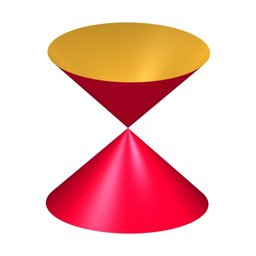
\includegraphics[width=1.4cm]{kegel}
        \end{tabular}
      \end{tabular}
    \end{center}
     المخروط المزدوج (الصورة إلى) هو اسهل المنحنيات المتفردة: إنه المتفرد الوحيد الذي يمكن وصفه بواسطة معادلة من الدرجة الثانية.
    \[x^2+y^2-z^2=0.\]
    عند تغيير هذه المعادلة بإستبدال الصفر بقيمة صغيرة $a\neq 0$، يتحول المخروط المزدوج إلى واحد من السطحين الزائدين أدناه، بحسب علامة $a$:
    \begin{center}
      \begin{tabular}{@{}c@{\ }c@{\ }c@{\ }c@{\ }c@{}}
        \begin{tabular}{@{}c@{}}
          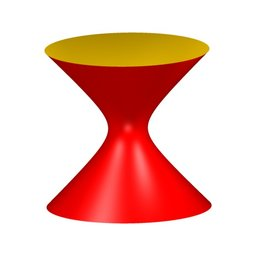
\includegraphics[width=1.2cm]{A1pm_2}
        \end{tabular}
        &
        $\leftarrow$
        &
        \begin{tabular}{@{}c@{}}
          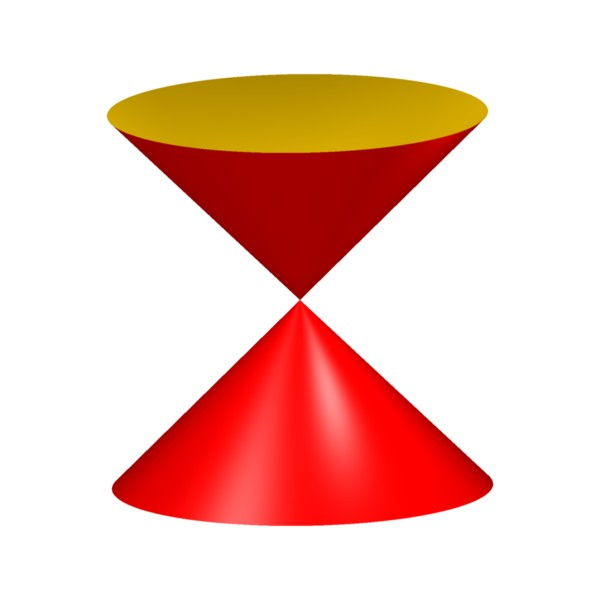
\includegraphics[width=1.2cm]{A1pm_1}
        \end{tabular}
        &
        $\rightarrow$
        &
        \begin{tabular}{@{}c@{}}
          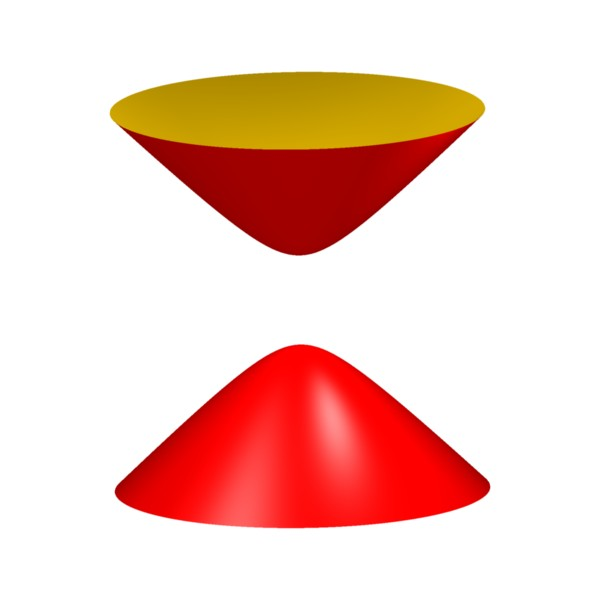
\includegraphics[width=1.2cm]{A1pm_0}
        \end{tabular}
      \end{tabular}
    \end{center}
  لا يمكن لسطح من الدرجة الثانية أن يملك أكثر من نقطة متفردة، هذا يعني أن \ $\mu(2)=1$
\end{surferPage}
